\documentclass{beamer}

\usepackage{mpemath}
\usepackage{subcaption}
\usepackage[normalem]{ulem}
\usepackage{amsmath}
\usepackage{amssymb}
\usepackage{mathtools}
%\usepackage{pgf}
%\usepackage{pgfplots}
%\usepackage{tikz}
\usepackage{booktabs}
\usepackage{siunitx}
\usepackage{natbib}
\usepackage{tabularx}
\usepackage{multirow}
\usepackage{amsmath}
\usepackage{mathtools}
\usepackage{amssymb}
\usepackage{bbm}
\usepackage[dvipsnames]{xcolor} % Saved my life during a conference once


%\usetikzlibrary{arrows,automata,backgrounds,positioning,decorations,intersections,matrix}

% *** Styles ***
\usetheme{Singapore}
\setbeamertemplate{navigation symbols}{}
% \usetheme[progressbar=frametitle]{metropolis}
% \usecolortheme{dolphin}
%\useinnertheme{circles}
%\usecolortheme{rose}
%\setbeamercovered{transparent}
\setbeamercovered{invisible}
\usefonttheme{professionalfonts}
%\usefonttheme[onlymath]{serif}
\setbeamertemplate{footline}[frame number]

\title{Mitigating the Curse of Horizon in Monte-Carlo Returns}
\author{Gersi Doko}
\institute{Department of Computer Science \\ University of New Hampshire}
\date{}

\AtBeginSection[]{
	\begin{frame}
          \vfill
	\centering
	% \usebeamerfont{title}
        {\huge\bf \insertsectionhead}%
	\vfill
\end{frame}
}

\begin{document}

\frame{\titlepage}

\section*{Intro}

\begin{frame}
\frametitle{MDP}
\begin{itemize}
  \item A Markov Decision Process (MDP) is a tuple $(S, A, f, R, \gamma, \eta)$
  \vfill
  \item Here we consider continuous MDPs, with deterministic transitions and rewards for simplicity
  \vfill
  \item $\frac{ds(t)}{dt} = f(s(t), a(t))$
\end{itemize}
\end{frame}

\begin{frame}
\frametitle{Monte-Carlo Returns Discrete Case}
  Very common to estimate the value of a policy by sampling returns over $M$ trajectories each of length $T$
  $[(s^m_t, a^m_t, r^m_t)_{t=0}^{T}]_{m=0}^{M}$
  \vfill
  $$\hat{G}_m^\pi = \sum_{t=0}^{T} \gamma^t \tilde{R}^m_{t}$$
  $$\hat{V}_M^\pi = \frac{1}{M} \sum_{m=0}^{M} \hat{G}_m^\pi$$
  \vfill
  \textbf{What is the relationship between $M$, $T$ and $\lvert\lvert \tilde{V}_\pi - V_\pi \rvert\rvert_1$?}
\end{frame}

\begin{frame}
\frametitle{Monte-Carlo Returns Continuous Case}
To investigate this question the paper considers the continuous time case,
\vfill
  $$G_T^\pi = \int_{0}^{T} \gamma^t r(s_t, \pi(s_t)) \; dt$$
  $$V_T^\pi = \mathbb{E}[G^\pi_T \mid s_0 \sim \eta]$$
\vfill
approximate the above integral over $T$ using discretization $N=[n_0, n_1, \dots]$
  $$\hat{G}_m^\pi = \sum_{n=0}^{N} \gamma^t \bar{r}^m_{n}$$
  $$\hat{V}^\pi_M = \frac{1}{M} \sum_{m=0}^{M} \hat{G}_m^\pi$$
\end{frame}

\begin{frame}
\frametitle{Monte-Carlo Returns Continuous Case}
  $$\bar{r}_m(n) = \frac{\gamma^{t_n} r_m(t_n) + \gamma^{t_{n-1}} r_m(t_{n-1})}{2}(t_n - t_{n-1})$$
  $$\hat{G}_m^\pi = \sum_{n=0}^{N} \gamma^t \bar{r}_m(n)$$
  $$\hat{V}^\pi_M = \frac{1}{M} \sum_{m=0}^{M} \tilde{G}_m^\pi$$
  \textbf{What is the relationship between $M$, $N$ and $\lvert\lvert \hat{V}^\pi_M - V_\pi \rvert\rvert_1$?}
\end{frame}

\section*{Goal}

\begin{frame}
  \frametitle{Goal}
  \begin{itemize}
    \item We have a fixed computation budget $B = M\cdot N$
    \item Want to minimize $\lvert\lvert \hat{V}^\pi_M - V_\pi \rvert\rvert_1$
    \vfill
    \item \textbf{How should we allocate $M$ and $N$?}
    \vfill
    \item \emph{Approach}: Allocate $N$ first, them $M = B/N$
  \end{itemize} 
\end{frame}

\section*{Algorithms}

\begin{frame}
	\frametitle{Adaptive}
  \begin{figure}[ht]
    \centering
    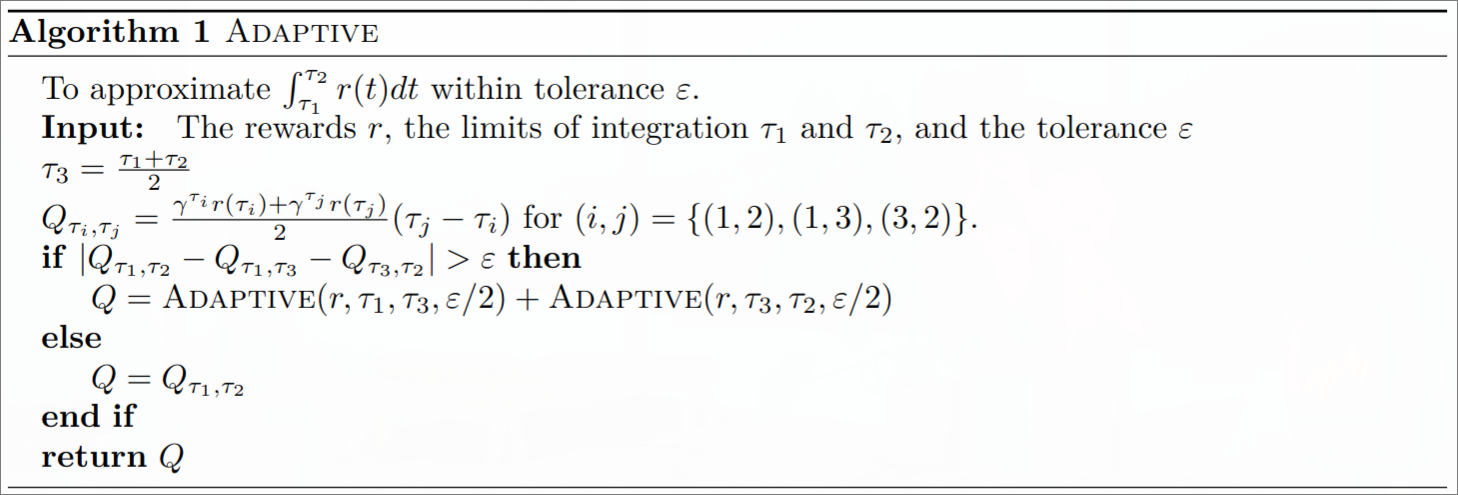
\includegraphics[width=\textwidth]{./imgs/adaptive.png} % Replace with your image file name
    \caption{Adaptive choice of discretization.}
  \end{figure}
\end{frame}

\begin{frame}
	\frametitle{Uniform}
  \begin{figure}[ht]
    \centering
    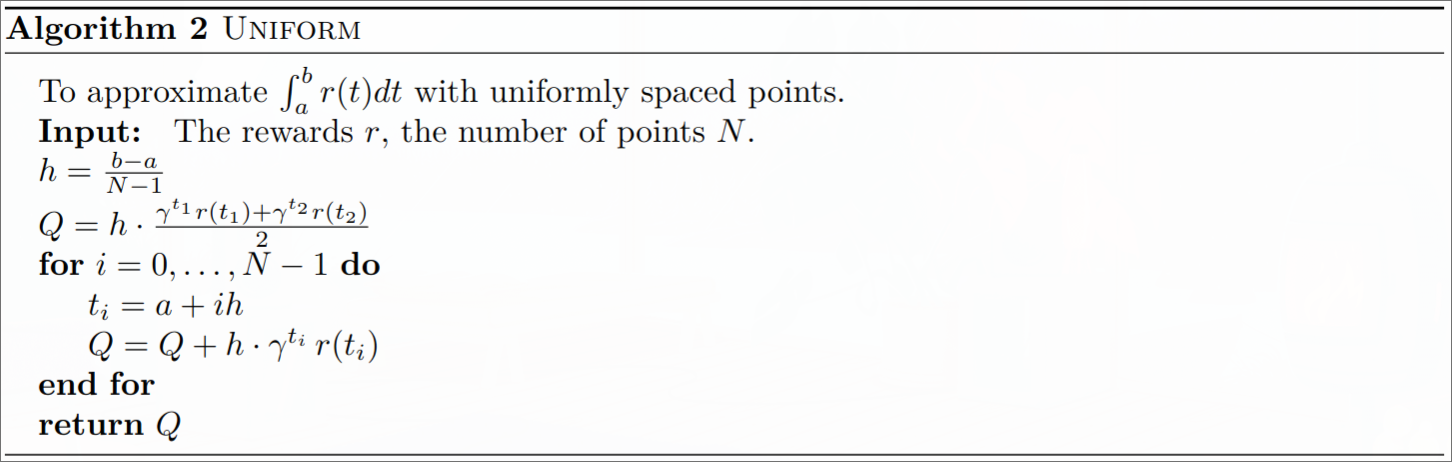
\includegraphics[width=\textwidth]{./imgs/uniform.png} % Replace with your image file name
    \caption{Uniform choice of discretization.}
  \end{figure}
\end{frame}

\section*{Experiments}
\begin{frame}
	\frametitle{Experiments}
  \begin{figure}[ht]
    \centering
    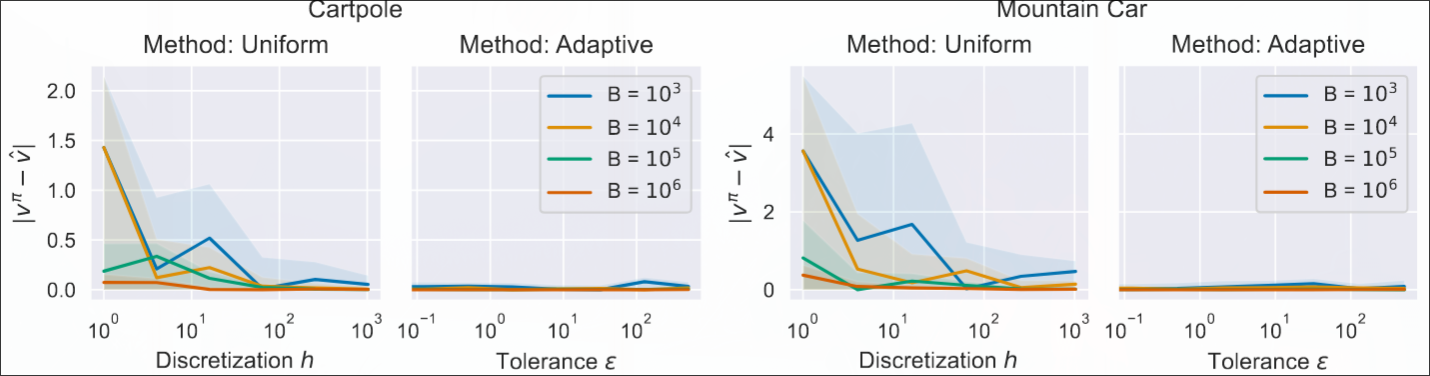
\includegraphics[width=\textwidth]{./imgs/experiments.png} % Replace with your image file name
    \caption{Experiments comparing Adaptive and Uniform discretization.}
  \end{figure}
\end{frame}

\begin{frame}
	\frametitle{Experiments Cont.}
  \begin{figure}[ht]
    \centering
    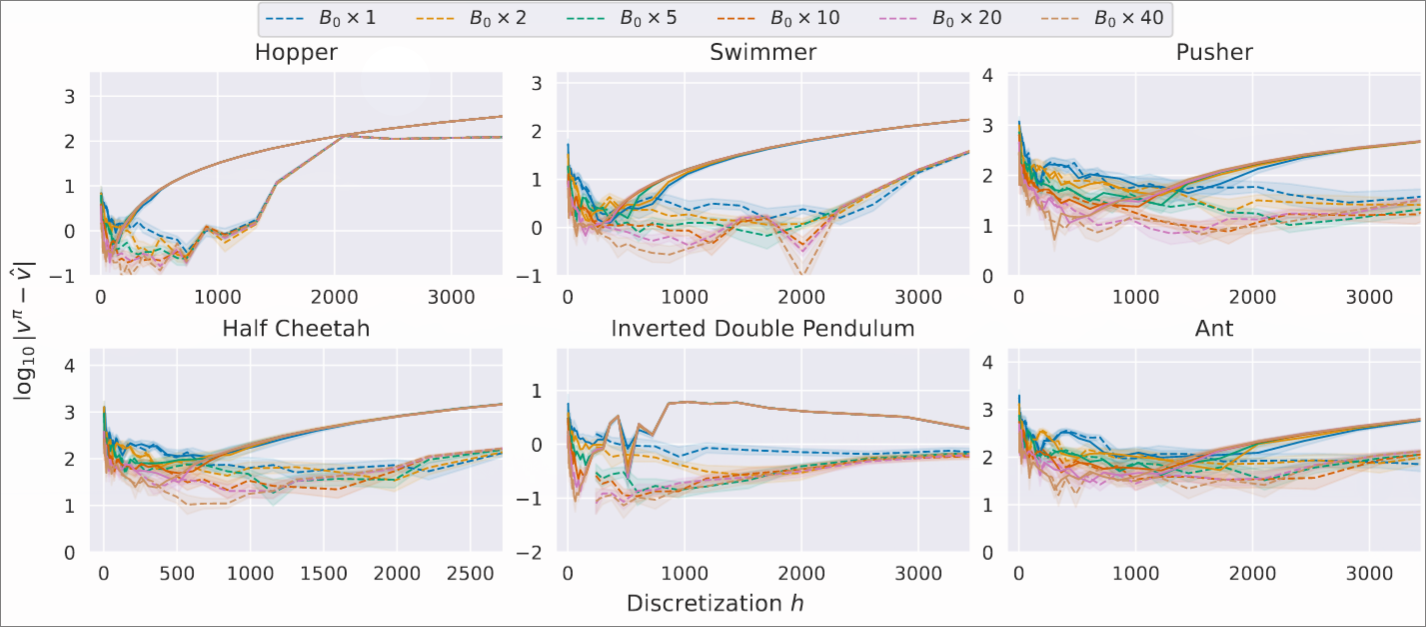
\includegraphics[width=\textwidth]{./imgs/experiments-mujoco.png} % Replace with your image file name
    \caption{Dashed line is adaptive, solid line is uniform.}
  \end{figure}
\end{frame}

\begin{frame}
	\frametitle{Conclusion}
  \begin{itemize}
    \item Don't always use all samples from Monte-Carlo rollouts
    \item Adaptive discretization is better than Uniform generally
    \item Better to use more samples with smaller discretization in uncertain regions of the state space
  \end{itemize}
\end{frame}

\end{document} 
